\documentclass[11pt]{article}
\usepackage[margin=1.0in]{geometry}
\usepackage{setspace}
\usepackage{amsmath}
\usepackage{fancyhdr}
\usepackage{listings}
\usepackage{tikz}
\pagestyle{fancy}
\lhead{CS 4610 Written Assignment 4}
\rhead{Zihao Wang (zw2rf)}
\cfoot{\thepage}
\renewcommand{\headrulewidth}{0.4pt}
\renewcommand{\footrulewidth}{0.4pt}
\renewcommand{\thesubsection}{\alph{subsection}.}
\lstset {
	language=C++,
	frame=single,
	numbers=left,
	backgroundcolor=\color{white}
}

\begin{document}
\thispagestyle{empty}
\title{CS 4610 Written Assignment 4}
\author{Zihao Wang (zw2rf)}
\date{\today}
\maketitle
\doublespacing

\section{Allowing multiple inheritance changes the way we define and use the least upper bound function on types}
\subsection{Explain, using at least one example why it is necessary to change \textit{lub}.}
Multiple inheritance makes the definition of least upper bound ambiguous. For example, consider the following inheritance tree: 
\begin{center}
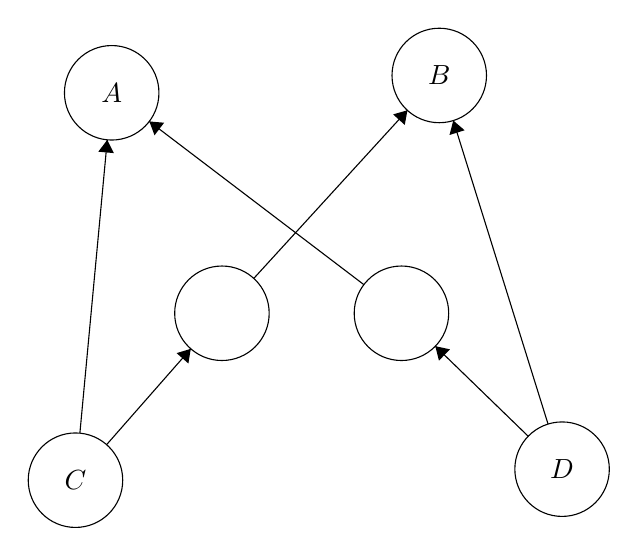
\begin{tikzpicture}[scale=0.2]
\tikzstyle{every node}+=[inner sep=0pt]
\draw [black] (26.8,-10.5) circle (3);
\draw (26.8,-10.5) node {$A$};
\draw [black] (24.5,-35.1) circle (3);
\draw (24.5,-35.1) node {$C$};
\draw [black] (33.8,-24.5) circle (3);
\draw [black] (47.6,-9.4) circle (3);
\draw (47.6,-9.4) node {$B$};
\draw [black] (55.4,-34.4) circle (3);
\draw (55.4,-34.4) node {$D$};
\draw [black] (45.2,-24.5) circle (3);
\draw [black] (24.78,-32.11) -- (26.52,-13.49);
\fill [black] (26.52,-13.49) -- (25.95,-14.24) -- (26.94,-14.33);
\draw [black] (26.48,-32.84) -- (31.82,-26.76);
\fill [black] (31.82,-26.76) -- (30.92,-27.03) -- (31.67,-27.69);
\draw [black] (35.82,-22.29) -- (45.58,-11.61);
\fill [black] (45.58,-11.61) -- (44.67,-11.87) -- (45.41,-12.54);
\draw [black] (54.51,-31.54) -- (48.49,-12.26);
\fill [black] (48.49,-12.26) -- (48.25,-13.18) -- (49.21,-12.88);
\draw [black] (53.25,-32.31) -- (47.35,-26.59);
\fill [black] (47.35,-26.59) -- (47.58,-27.51) -- (48.28,-26.79);
\draw [black] (42.81,-22.68) -- (29.19,-12.32);
\fill [black] (29.19,-12.32) -- (29.52,-13.2) -- (30.13,-12.4);
\end{tikzpicture}
\end{center}
If we want to find \textit{lub}(C, D), both class A and class B are equivalent answers. 

\subsection{Describe how you want to implement \textit{lub} for multiple inheritance.}
Firstly, we must allow \textit{lub} operation to return a list of classes instead of just one. To find such a list of least upper bounds, do the normal operation of \textit{lub} and sort the results by the sum of total number of parent classes taken for both classes to get to that specific common parent class. Return the list of classes containing least sums in that list. 

\section{Add code to the \lstinline|main| method so that the resulting program is a valid Java program, but running that program triggers one of the aforementioned runtime checks.}
\begin{lstlisting}
class Mammal { String name; }
class Dog extends Mammal {
	void beginBarking() { ... }
}
class Main {
	public static void main (String argv[]) {
		Dog x[] = new Dog[5];
		Mammal y[] = x;
		for  (int i = 0; i < y.length; y++) {
			y[i].beginBarking();
		}
	}
}
\end{lstlisting}
This code will trigger run-time checks to determine the dynamic types of the array of \lstinline|Mammal|. Since the method \lstinline|beginBarking()| is only defined in \lstinline|Dog|, we have to check the dynamic types.

\setcounter{subsection}{0}

\section{List the flaws and explain how they affect the judgement}
\subsection{\textit{let-init}}
\begin{itemize}
\item $O \vdash e_{1} : T_{1}$ should be $O[x/T_{0}] \vdash e_{1} : T_{1}$. This is because the let binding should be added to the map to evaluate the type of expression of $T_{1}$
\item $O[x/T_{0}] \vdash \text{ let } x : T_{0} \leftarrow e_{0} \text{ in } e_{1} : T_{1}$ should be $O \vdash \text{ let } x : T_{0} \leftarrow e_{0} \text{ in } e_{1} : T_{1}$. This is because the condition $x$ is of type $T_{0}$ is not necessary here.
\end{itemize}

\subsection{\textit{assign}}
\begin{itemize}
\item $T_{0} \le T_{1}$ should be $T_{1} \le T_{0}$. This is because the assignment expression should be a subtype of its declared type otherwise it is not safe.  
\end{itemize}

\subsection{\textit{self-type}}
\begin{itemize}
\item The condition for this rule should be $C \le T$ instead of $ T \le C $. Since $\text{SELF\_TYPE}_{C} $ refers to type C and any subtype of C. The conclusion $\text{SELF\_TYPE}_{C} \le T$ only works if $C \le T$
\end{itemize}

\subsection{\textit{static-dispatch-self}}
\begin{itemize}
\item Since this is static dispatch, the condition $M(T_{0}, f) = (T_{1}', ..., T_{n}', T_{n+1}')$ should be the casted type $M(T, f) = (T_{1}', ..., T_{n}', T_{n+1}')$.
\item if $T_{n+1}' = \text{SELF\_TYPE}$, the return type should be the type of $T_{0}$.
\end{itemize}

\end{document}